模板是C++的特性,这样函数和类可以支持泛型——可以实现独立于特定数据类型的函数或类,例如:客户端可以使用max()函数来处理不同的数据类型。不需要使用函数重载来实现和维护许多类似的函数,我们只需要实现一个max()并将数据类型作为参数传递。此外,模板可以与多重继承和操作符重载一起工作,从而在C++中可以创建强大的通用数据结构和算法,如:标准模板库(STL)。此外,模板还可以应用于编译时计算、编译时和运行时代码优化等。 \par
本章中,我们将学习函数和类模板的语法、它们的实例化和特化。然后,我们将介绍可变参数模板及其应用。接下来,将讨论模板参数和用于实例化它们的相应参数。之后,将学习如何实现一个类型特征,以及如何使用这种信息来优化算法。最后,将介绍一些可以用来提高程序执行速度的技术,包括编译时计算、编译时代码优化和静态多态性。\par
本章中,我们将了解以下内容: \par

\begin{itemize}
	\item 探索函数和类模板
	\item 了解可变模板
	\item 理解模板形参和参数
	\item 什么是特征?
	\item 模板元编程及其应用
\end{itemize}

\noindent\textbf{}\ \par
\textbf{源码位置} \ \par
本章的代码可以在这本书的GitHub中找到: https:/​/​github.com/​PacktPublishing/​Expert-​CPP . \par

\noindent\textbf{}\ \par
\textbf{探索函数和类模板} \ \par
我们将从介绍函数模板的语法开始,并通过实例化、推断类型和特化开始这一节。然后,我们将转向类模板,看看类似的概念,以及示例。\par

\noindent\textbf{}\ \par
\textbf{动机} \ \par
目前为止,定义了函数或类时,必须提供输入、输出和中间参数。例如,有一个函数来执行两个int型整数的加法运算。如何扩展它,使它能够处理所有其他基本数据类型,如float、double、char等?一种方法是通过手动复制、粘贴和稍微修改每个函数来使用函数重载。另一种方法是定义一个宏来执行加法操作。这两种方法都有各自的副作用。 \par
此外,如果我们修复了一个bug或为一种类型添加了一个新特性,而这个更新需要对所有其他重载函数和类执行,这会导致什么情况?除了使用复制-粘贴-替换的方法,有更好的方法来处理这种情况吗? \par
事实上,这是任何计算机语言都可能面临的问题。这个问题由通用函数编程元语言(ML,Meta Language)在1973年提出,ML允许编写仅在使用时的类型集中使用不同的通用函数或类型,从而减少重复代码。后来,受Ada语言中特定生命保证(CLU,hartered life underwriter)提供的参数化模块和泛型的启发,C++采用了模板概念,它允许函数和类使用泛型类型进行操作。换句话说,它允许函数或类处理不同的数据类型,而不需要重新编写它们。 \par
实际上,从抽象的角度来看,C++函数或类模板可以作为创建其他类似函数或类的模式。这背后的基本思想是创建一个函数或类模板,而不必指定某些或所有变量的确切类型。我们使用占位符类型定义函数或类模板,称为模板类型形参。一旦有了函数或类模板,就可以使用在其他编译器中实现的算法自动生成函数或类。 \par
C++中有三种模板:函数模板、类模板和可变参数模板。接下来我们一个个的来了解。 \par

\noindent\textbf{}\ \par
\textbf{函数模板} \ \par
函数模板定义了如何生成一系列函数。这里是指一组行为相似的函数。如下图所示,这包括两个阶段: \par

\begin{itemize}
	\item 创建函数模板,如何书写的规则。
	\item 模板实例化,从模板中生成函数的规则:
\end{itemize}

\begin{center}
	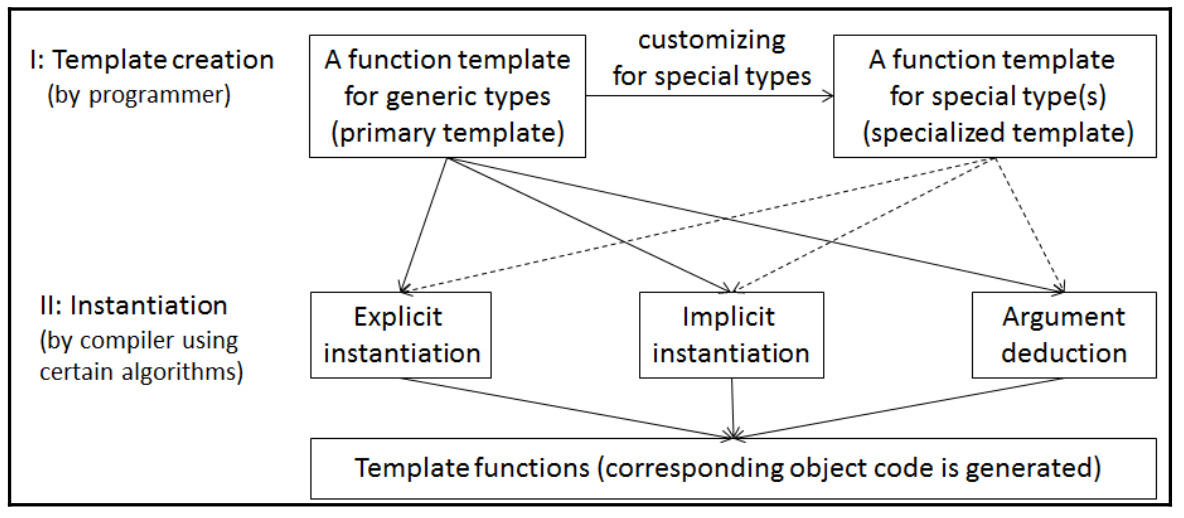
\includegraphics[width=0.6\textwidth]{content/Section-1/Chapter-4/1}
\end{center}

上图的第一部分中,讨论了用于为泛型类型创建函数模板的格式,但与特化模板有关,我们也将特化模板称为主模板。第二部分中,我们介绍从模板生成函数的三种方法。最后,特化和重载小节告诉我们如何为特殊类型定制主模板(通过改变其行为)。 \par

\noindent\textbf{}\ \par
\textbf{语法} \ \par
定义函数模板有两种方法,如下面的代码所示: \par

\begin{lstlisting}[caption={}]
template <typename identifier_1, …, typename identifier_n >
function_declaration;

template <class identifier_1,…, class identifier_n>
function_declaration;
\end{lstlisting}

这里,\texttt{identifier\underline{ }i (i=1,…,n)}是类型或类形参,而function\underline{ }declaration声明了部分函数体。前面两个声明的唯一区别是关键字——一个使用class,另一个使用typename,两者具有相同的含义和行为。因为类型(例如基本类型——int、float、double、enum、struct、union等)不是类,所以引入了typename关键字方法以避免混淆。 \par
例如,查找最大值函数模板app\underline{ }max()可以这样声明: \par

\begin{lstlisting}[caption={}]
template <class T>
T app_max (T a, T b) {
	return (a>b?a:b); //note: we use ((a)>(b) ? (a):(b)) in macros
}                     //it is safe to replace (a) by a, and (b) by b now
\end{lstlisting}

这个函数模板可以用于许多数据类型或类,只要有一个可复制构造的类型,其中表达式是a>b。对于用户定义的类,这意味着必须定义大于操作符(>)。 \par
注意,函数模板和模板函数是不同的东西。函数模板是一种编译器用来生成函数的模板,因此编译器不会为它生成任何目标代码。另一方面,模板函数是指函数模板中的一个实例。由于它是一个函数,相应的目标代码由编译器生成。然而,最新的C++标准文档建议避免使用不精确的术语定义模板函数。因此,本书中将使用函数模板和成员函数模板。 \par

\noindent\textbf{}\ \par
\textbf{实例化} \ \par
因为可能有无限多个类型和类,函数模板的概念不仅节省了源代码的空间,而且使代码更容易阅读和维护。然而,与为应用程序中使用的不同数据类型编写单独的函数或类相比,模板不会产生更小的目标代码。例如,考虑一个使用float和int版本的app\underline{ }max()的程序: \par

\begin{lstlisting}[caption={}]
cout << app_max<int>(3,5) << endl;
cout << app_max<float>(3.0f,5.0f) << endl;
\end{lstlisting}

编译器将在目标文件中生成两个新函数,如下所示:\par

\begin{lstlisting}[caption={}]
int app_max<int> ( int a, int b) {
	return (a>b?a:b);
}

float app_max<float> (float a, float b) {
	return (a>b?a:b);
}
\end{lstlisting}

从函数模板声明创建函数的过程称为模板实例化。这个实例化过程中,编译器确定模板参数,并根据应用程序的需要生成实际的函数代码。实例化通常有三种形式:显式、隐式和推断。我们接下来讨论每一种形式。 \par

\noindent\textbf{}\ \par
\textbf{显式实例化} \ \par
很多非常有用的C++函数模板可以在不使用显式实例化的情况下编写和使用,将在这里描述它们,以便在需要时知道它们的存在。首先,看一下C++11之前显式实例化的语法。有两种形式,代码如下所示: \par

\begin{lstlisting}[caption={}]
template return-type
function_name < template_argument_list > ( function_parameter-list );

template return-type
function_name ( function_parameter_list );
\end{lstlisting}

显式实例化定义,强制对特定类型的函数模板进行实例化,而不管将来会调用哪个模板函数。显式实例化可以在函数模板定义之后的任何位置,并且对于源代码中的给定参数列表,它只允许出现一次。 \par
自C++11以来,显式实例化的语法如下所示,我们可以看到关键字extern放在关键字template之前: \par

\begin{lstlisting}[caption={}]
extern template return-type
function_name < template_argument_list > (function_parameter_list ); \\ (since C++11)

extern template return-type
function_name ( function_parameter_list ); \\ (since C++11)
\end{lstlisting}

使用extern关键字可以防止隐式实例化该函数模板(参阅下一节)。 \par
前面声明的app\underline{ }max()函数模板,可以使用以下代码显式实例化: \par

\begin{lstlisting}[caption={}]
template double app_max<double>(double, double);
template int app_max<int>(int, int);
\end{lstlisting}

也可以使用以下代码显式实例化: \par

\begin{lstlisting}[caption={}]
extern template double app_max<double>(double, double); //(since c++11)
extren template int app_max<int>(int, int); //(since c++11)
\end{lstlisting}

也可以通过模板参数推导的方式完成: \par

\begin{lstlisting}[caption={}]
template double f(double, double);
template int f(int, int);
\end{lstlisting}

最后,也可以这样做: \par

\begin{lstlisting}[caption={}]
extern template double f(double, double); //(since c++11)
extern template int f(int, int); //(since c++11)
\end{lstlisting}

此外,还有一些用于显式实例化的规则。如果想了解更多,请参考扩展阅读部分的[10]了解更多信息。 \par

\noindent\textbf{}\ \par
\textbf{隐式实例化} \ \par
当一个函数调用时,该函数的定义必须存在。如果这个函数没有显式实例化,则会进行隐式实例化。隐式实例化中,模板参数列表需要显式地提供或从上下文推导出来参数类型。下面程序的A部分提供了app\underline{ }max()隐式实例化的例子: \par

\begin{lstlisting}[caption={}]
//ch4_2_func_template_implicit_inst.cpp
#include <iostream>
template <class T>
T app_max (T a, T b) { return (a>b?a:b); }
using namespace std;
int main(){
	//Part A: implicit instantiation in an explicit way
	cout << app_max<int>(5, 8) << endl; //line A
	cout << app_max<float>(5.0, 8.0) << endl; //line B
	cout << app_max<int>(5.0, 8) << endl; //Line C
	cout << app_max<double>(5.0, 8) << endl; //Line D
	//Part B: implicit instantiation in an argument deduction way
	cout << app_max(5, 8) << endl; //line E
	cout << app_max(5.0f, 8.0f) << endl; //line F
	//Part C: implicit instantiation in a confuse way
	//cout<<app_max(5, 8.0)<<endl; //line G
	return 0;
}
\end{lstlisting}

行A、B、C和D的隐式实例化分别为int app\underline{ }max<int>(int,int)、float app\underline{ }max<float>(float, float>)、int app\underline{ }max<int>(int,int)和double app\underline{ }max<double>(double, double)。 \par

\noindent\textbf{}\ \par
\textbf{类型推断} \ \par
当调用模板函数时,即使不是每个模板实参都指定了,编译器也需要找出具体的实参。大多数情况下,它会从函数参数中推断出缺少的模板参数。例如,在前面函数的B部分中,当在E行中调用app\underline{ }max(5,8)时,编译器将模板实参推断为int类型(int app\underline{ }max<int>(int,int)),因为输入形参5和8都是整数。类似地,行F将被推断为float类型,即float app\underline{ }max<float>(float,float)。 \par
如果在实例化过程中出现混乱怎么办?例如,前一个程序的G注释掉的行中,根据编译器的不同,可以调用app\underline{ }max<double>(double, double), app\underline{ }max<int>(int, int),或者抛出编译错误消息。帮助编译器推断类型的最好方法是通过显式地给出模板实参来调用函数模板。这种情况下,如果调用app\underline{ }max<double>(5,8.0),任何混淆都将得到解决。 \par

\hspace*{\fill} \\ %插入空行

\includegraphics[width=0.05\textwidth]{images/tip}
从编译器的角度来看,有几种方法可以进行模板参数推断——从函数调用推断、从类型推断、自动类型推断和上下文[4]。然而,从开发者角度来看,你永远不应该编写花哨的代码来使用函数模板演绎的概念来迷惑其他程序员,比如前面的例子中的第G行。\par
\noindent\textbf{}\ \par

\noindent\textbf{}\ \par
\textbf{特化和重载} \ \par
特化允许为一组给定的模板实参定制模板代码,允许我们为特定的模板参数定义特定的行为。特化仍然是模板,仍然需要实例化来获得真正的代码(由编译器自动完成)。\par
下面的示例代码中,主函数模板\texttt{T app\underline{ }max(T a, T b})将根据操作符a>b返回a或b,可以将其特化为\texttt{T = std::string},这样我们只比较a和b的第0个元素,即a[0] >b[0]就可以了: \par

\begin{lstlisting}[caption={}]
//ch4_3_func_template_specialization.cpp
#include <iostream>
#include <string>
//Part A: define a primary template
template <class T> T app_max (T a, T b) { return (a>b?a:b); }
//Part B: explicit specialization for T=std::string,
template <>
std::string app_max<std::string> (std::string a, std::string b){
	return (a[0]>b[0]?a:b);
}
//part C: test function
using namespace std;
void main(){
	string a = "abc", b="efg";
	cout << app_max(5, 6) << endl; //line A
	cout << app_max(a, b) << endl; //line B
	//question: what's the output if un-comment lines C and D?
	//char *x = "abc", *y="efg"; //Line C
	//cout << app_max(x, y) << endl; //line D
}
\end{lstlisting}

前面的代码定义了主模板,然后显式特化为std::string,我们不比较a和b的值,只关心a[0]和b[0] (app\underline{ }max()的行为是特化的)。在测试函数中,行A调用app\underline{ }max<int>(int,int),行B调用专用版本,因为在推导时没有歧义。如果取消注释C和D行,则会调用主函数模板\texttt{char* app\underline{ }max<char> (char*, char*)},因为char*和std::string是不同的数据类型。 \par
本质上,特化与函数重载有些冲突:编译器需要一种算法来解决这种冲突,方法是在模板和重载函数之间找到正确的匹配。选择正确函数的算法包括以下两个步骤: \par

\begin{enumerate}
	\item 常规函数和非特化模板之间执行重载解析。
	\item 如果选择了非特化模板,请检查是否存在与之更匹配的特化模板。
\end{enumerate}

例如,下面的代码块中,我们声明了主函数(第0行)和特化函数模板(第1-4行),以及f()的重载函数(第5-6行): \par

\begin{lstlisting}[caption={}]
template<typename T1, typename T2> void f( T1, T2 );// line 0
template<typename T> void f( T ); // line 1
template<typename T> void f( T, T ); // line 2
template<typename T> void f( int, T* ); // line 3
template<> void f<int>( int ); // line 4
void f( int, double ); // line 5
void f( int ); // line 6
\end{lstlisting}

f()将在下面的代码块中多次调用。根据前面的两步规则,可以在注释中显示选择了哪个函数。我们将在下面解释这样做的原因: \par

\begin{lstlisting}[caption={}]
int i=0;
double d=0;
float x=0;
complex<double> c;
f(i); //line A: choose f() defined in line 6
f(i,d); //line B: choose f() defined in line 5
f<int>(i); //line C: choose f() defined in line 4
f(c); //line D: choose f() defined in line 1
f(i,i); //line E: choose f() defined in line 2
f(i,x); //line F: choose f() defined in line 0
f(i, &d); //line G: choose f() defined in line 3
\end{lstlisting}

对于直线A和直线B,由于第5行和第6行定义的f()是常规函数,它有最高的优先级,因此f(i)和f(i,d)将选择它。对于行C,因为特化模板存在,所以从第4行生成的f()比从第1行创建的f()更匹配。对于第D行,因为c是一个complex<double>类型,只有第1行中定义的主函数模板匹配它。E行选择第2行创建的f(),因为这两个输入变量是同一类型的。最后,第F行和第G行将分别从第0行和第3行模板中获取函数。 \par
了解了函数模板之后,来看看类型模板。 \par

\noindent\textbf{}\ \par
\textbf{类型模板} \ \par
类模板定义了一系列类,通常用于实现容器。例如,C++标准库包含许多类模板,如std::vector、std::map、std::deque等。OpenCV中,cv::Mat是一个非常强大的类模板,可以处理带有内置数据类型如int8\underline{ }t、uint8\underline{ }t、int16\underline{ }t、uint16\underline{ }t、uint32\underline{ }t、uint32\underline{ }t、float、double等的1D、2D和3D矩阵或图像。 \par
类似于函数模板,如下图所示,类模板的概念包含一个模板创建语法,它的特化,以及它的隐式和显式实例化: \par

\begin{center}
	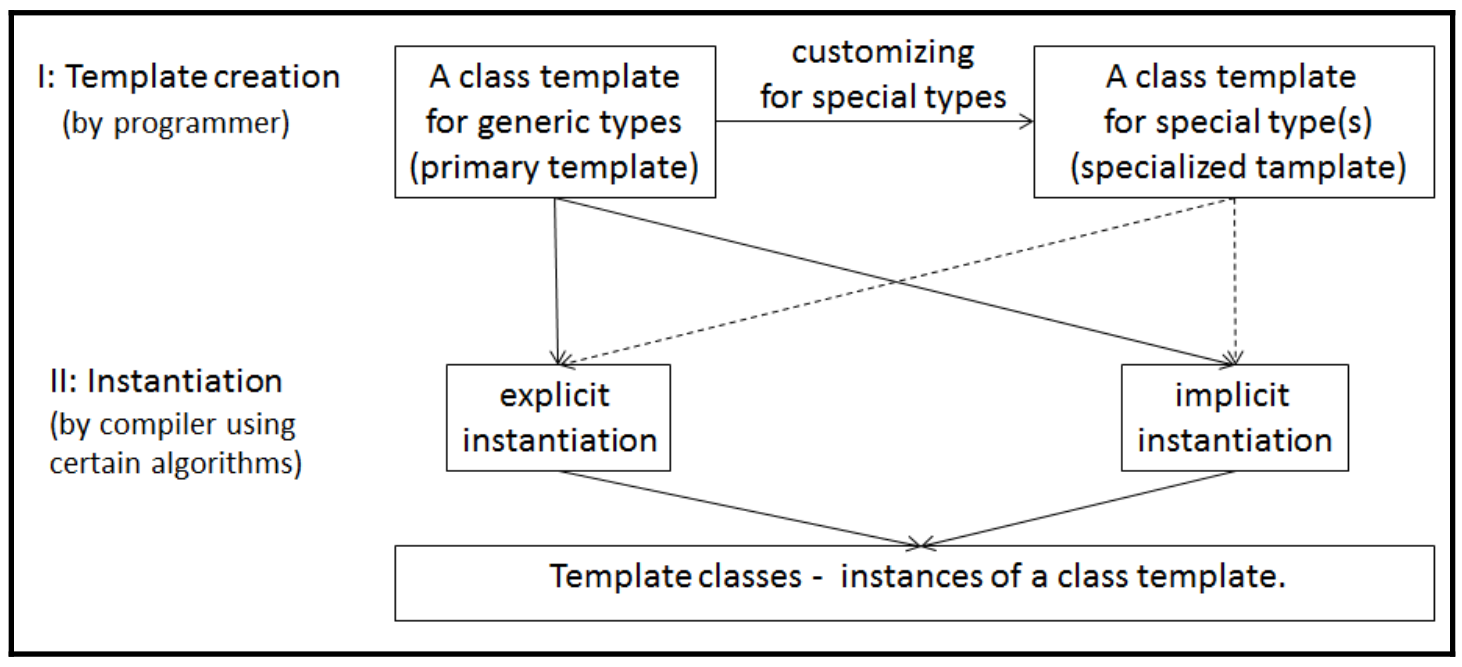
\includegraphics[width=0.6\textwidth]{content/Section-1/Chapter-4/2}
\end{center}

图的\textbf{part I}中,使用特定的语法格式,可以为泛型类型创建类模板,也称为主模板,并且可以为具有不同成员函数和/或变量的特殊类型定制。\textbf{part II}中,当我们有了类模板,编译器就会根据应用程序的需求显式或隐式地将模板实例化。\par
现在,了解一下创建类模板的语法。 \par

\noindent\textbf{}\ \par
\textbf{语法} \ \par
创建类模板的语法如下: \par

\begin{lstlisting}[caption={}]
[export] template <template_parameter_list> class-declaration
\end{lstlisting}

这里,我们有以下这些方式: \par

\begin{itemize}
	\item \texttt{template\underline{ }parameter-list}(请参阅进一步阅读上下文[10]中的链接)是一个非空的以逗号分隔的模板形参列表,每个模板形参要么是一个非类型形参,要么是一个类型形参,或是一个模板形参。
	\item \texttt{class-declaration}用来声明类,这个类包含一个类名和用花括号括起来的类体。通过这样做,声明的类名也变成了模板名。
\end{itemize}

例如,可以定义一个类模板V,使其包含各种1D数据类型:\par

\begin{lstlisting}[caption={}]
template <class T>
class V {
public:
	V( int n = 0) : m_nEle(n), m_buf(0) { creatBuf();}
	~V(){ deleteBuf(); }
	V& operator = (const V &rhs) { /* ... */}
	V& operator = (const V &rhs) { /* ... */}
	T getMax(){ /* ... */ }
protected:
	void creatBuf() { /* ... */}
	void deleteBuf(){ /* ... */}
public:
	int m_nEle;
	T * m_buf;
};
\end{lstlisting}

有了这个类模板,编译器就可以在实例化过程中生成类。由于在函数模板小节中提到的原因,本书中我们将避免使用不精确的术语定义模板类。 \par

\noindent\textbf{}\ \par
\textbf{实例化} \ \par
回顾一下上一节定义的类模板V,假设后面会出现以下声明: \par

\begin{lstlisting}[caption={}]
V<char> cV;
V<int> iV(10);
V<float> fV(5);
\end{lstlisting}

然后,编译器将创建V类的三个实例,如下所示: \par

\begin{lstlisting}[caption={}]
class V<char>{
public:
	V(int n=0);
	// ...
public:
	int m_nEle;
	char *m_buf;
};
class V<int>{
public:
	V(int n=0);
	// ...
public:
	int m_nEle;
	int *m_buf;
};
class V<float>{
public:
	V(int n = 0);
	// ...
public:
	int m_nEle;
	float *m_buf;
};
\end{lstlisting}

与函数模板实例化类似,类模板实例化有两种形式:显式和隐式。 \par

\noindent\textbf{}\ \par
\textbf{显式实例化} \ \par
显式实例化的语法如下: \par

\begin{lstlisting}[caption={}]
template class template_name < argument_list >;
extern template class template_name < argument_list >;//(since C++11)
\end{lstlisting}

显式实例化定义强制实例化的所引用的类、结构体或联合体。C++11标准中,模板特化或其成员的隐式实例化将被抑制。与函数模板的显式实例化类似,该显式实例化的位置可以在其模板定义之后的任何位置,并且只允许在整个程序的一个文件中定义。\par
而且,由于C++11隐式实例化将显式的声明(extern模板)绕过。这可以用来减少编译时间。 \par 
回到模板类V,我们可以显式地实例化它: \par

\begin{lstlisting}[caption={}]
template class V<int>;
template class V<double>;
\end{lstlisting}

或者,我们可以这样做(从C++11开始): \par

\begin{lstlisting}[caption={}]
extern template class V<int>;
extern template class V<double>;
\end{lstlisting}

如果显式实例化一个函数或类模板,但在程序中没有相应的定义,编译器将报出错误消息,如下所示: \par

\begin{lstlisting}[caption={}]
//ch4_4_class_template_explicit.cpp
#include <iostream>
using namespace std;
template <typename T> //line A
struct A {
	A(T init) : val(init) {}
	virtual T foo();
	T val;
}; //line B
//line C
template <class T> //T in this line is template parameter
T A<T>::foo() { //the 1st T refers to function return type,
	//the T in <> specifies that this function's template
	//parameter is also the class template parameter
	return val;
} //line D
extern template struct A<int>; //line E
#if 0 //line F
int A<int>::foo() {
	return val+1;
}
#endif //line G
int main(void) {
	A<double> x(5);
	A<int> y(5);
	cout<<"fD="<<x.foo()<<",fI="<<y.foo()<< endl;
	return 0; //output: fD=5,fI=6
}
\end{lstlisting}

前面的代码中,在A行和B行之间定义了一个类模板,然后从C行到D行实现了成员函数foo()。接下来,在E行为int类型显式实例化。由于在F行和G行之间的代码块注释掉了(这意味着对于这个显式的int类型实例化没有相应的foo()定义),我们有看到了链接错误。为了解决这个问题,我们需要在F行用\texttt{\#if 1}替换\texttt{\#if 0}。\par
最后,对于显式实例化声明还有一些限制: \par

\begin{itemize}
	\item \textbf{静态函数}:可以命名静态类成员,但不能在显式实例化声明中指定静态函数。
	\item \textbf{内联函数}:显式实例化声明中对内联函数没有影响,而内联函数是隐式实例化的。
	\item \textbf{类及其成员}:显式实例化类及其所有成员并不等价。
\end{itemize}

\noindent\textbf{}\ \par
\textbf{隐式实例化} \ \par


\noindent\textbf{}\ \par
\textbf{特化} \ \par

\noindent\textbf{}\ \par
\textbf{了解可变模板} \ \par

\noindent\textbf{}\ \par
\textbf{语法} \ \par

\noindent\textbf{}\ \par
\textbf{例子} \ \par

\noindent\textbf{}\ \par
\textbf{探索模板形参和参数} \ \par

\noindent\textbf{}\ \par
\textbf{模板参数} \ \par

\noindent\textbf{}\ \par
\textbf{实模板参数} \ \par

\noindent\textbf{}\ \par
\textbf{模板参数类型} \ \par

\noindent\textbf{}\ \par
\textbf{模板模板参数} \ \par

\noindent\textbf{}\ \par
\textbf{模板参数} \ \par

\noindent\textbf{}\ \par
\textbf{模板非类型参数} \ \par

\noindent\textbf{}\ \par
\textbf{模板类型参数} \ \par

\noindent\textbf{}\ \par
\textbf{模板的模板参数} \ \par

\noindent\textbf{}\ \par
\textbf{默认模板参数} \ \par

\noindent\textbf{}\ \par
\textbf{探索特征} \ \par

\noindent\textbf{}\ \par
\textbf{类型特征实现} \ \par

\noindent\textbf{}\ \par
\textbf{boost::is\underline{ }void} \ \par

\noindent\textbf{}\ \par
\textbf{boost::is\underline{ }pointer} \ \par

\noindent\textbf{}\ \par
\textbf{利用特征优化算法} \ \par

\noindent\textbf{}\ \par
\textbf{探索模板元编程} \ \par

\noindent\textbf{}\ \par
\textbf{编译时计算} \ \par

\noindent\textbf{}\ \par
\textbf{编译时优化} \ \par

\noindent\textbf{}\ \par
\textbf{静态多态性} \ \par

\noindent\textbf{}\ \par
\textbf{总结} \ \par

\noindent\textbf{}\ \par
\textbf{问题} \ \par

\noindent\textbf{}\ \par
\textbf{扩展阅读} \ \par

\newpage